\section{Motorparameters}

De \gls{AX5140} drive die in de testkast zit heeft 465 parameters, echter zijn er slechts een aantal relevant die aangepast moeten worden wanneer er een motor wordt gewisseld. Dit is bij synchrone servo motoren anders dan bij asynchrone servo motoren. Voortman gebruikt zowel synchrone als asynchrone servo motoren en daarom moet er in kaart gebracht worden welke parameters er veranderd moeten worden in geval van welke motor.

\vspace{0.5cm}

Om het voor de gebruiker wat makkelijker te maken heeft Beckhoff de drive manager 2 ontwikkeld hiermee is het vrij gemakkelijk om te zien welke parameters er relevant zijn voor welke type motor. Dit is bijvoorbeeld de lijst met parameters die ingevuld moeten worden bij een asynchrone roterende servo motor.

\begin{figure}[H]
	\centering
	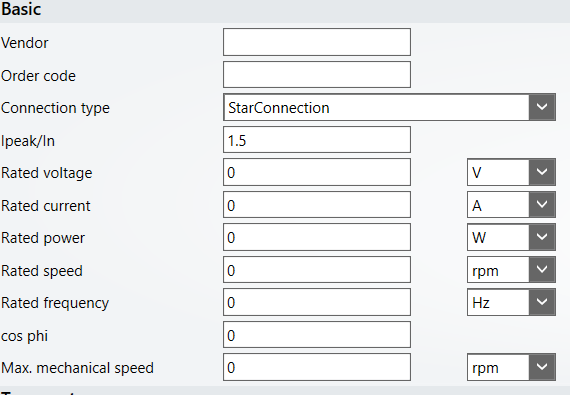
\includegraphics[width=300pt]{AsyncMotor}
	\label{fig:AsyncMotor}
	\caption{Parameter lijst voor een asynchrone roterende servo motor}
\end{figure}

Voor een synchrone servo motor wordt de parameter lijst een stukje langer maar deze is alsnog grotendeels hetzelfde. Deze parameters zijn over het algemeen allemaal bekend in de datasheet van de motor. Naast dat de parameters van de motor moeten worden gespecificeerd is het ook noodzakelijk om de massatraagheid in te vullen van de motor as en van de toolspindel zelf dit kan worden gehaald uit de datasheet van de motor en toolspindel van de fabrikant.

\begin{figure}[H]
	\centering
	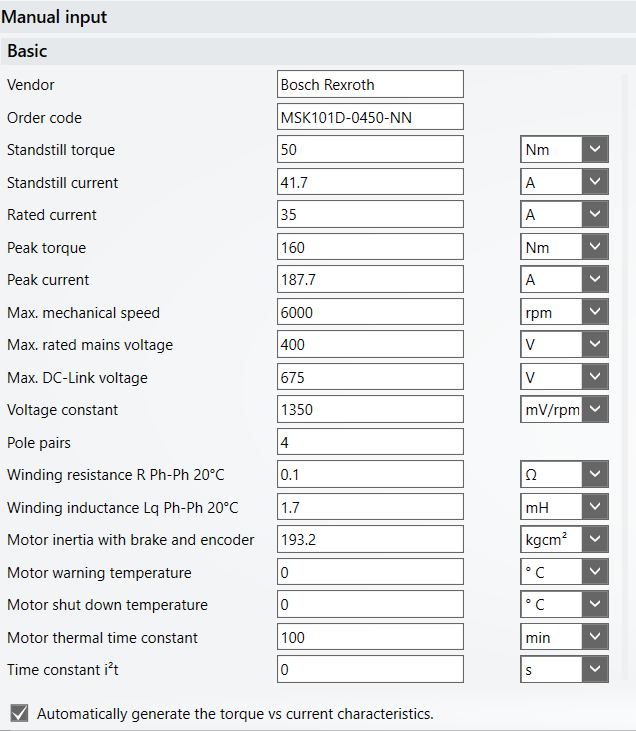
\includegraphics[width=300pt]{SyncMotor}
	\label{fig:SyncMotor}
	\caption{Parameter lijst voor een synchrone roterende servo motor}
\end{figure}

\begin{figure}[H]
	\centering
	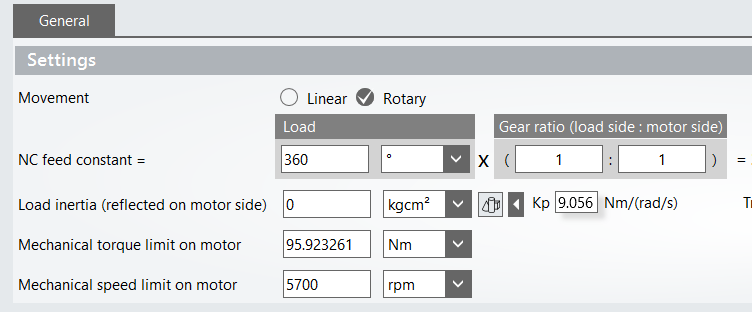
\includegraphics[width=300pt]{MotorLoad}
	\label{fig:MotorLoad}
	\caption{Motor belasting}
\end{figure}

Wanneer de gebruiker de parameter set wil verwisselen met een parameter set van een andere motor zou dit met één druk op de knop moeten kunnen het is daarom niet mogelijk om dit allemaal via de driver manager te doen. Het inladen van de nieuwe parameter set zal via TwinCAT ingeladen moeten worden hiervoor moet er uitgezocht worden welke IDN elke essentiële parameter heeft met de grootte van de parameter erbij zodat deze uitgelezen kunnen worden uit de drive en ook makkelijk weer geschreven kunnen worden. Zo kan een engineer wanneer er een nieuwe motor is deze motor fijn afstellen in de drive manager waarna het programma deze instellingen kan uitlezen in het programma van de testkast zodat er gemakkelijk kan worden gewisseld tussen de parameter sets.

\subsection{Statische variabelen}

Er zijn een aantal parameters die éénmaal gekozen moeten worden maar hierna eigenlijk niet meer veranderd hoeven te worden. Wel is het verstandig om deze op te slaan in de parameter lijst mocht de drive een keer compleet resetten dan hoeft de gebruiker deze niet handmatig te schrijven:

\begin{enumerate}
	\item \textbf{P-0-2000 Geconfigureerde veiligheidsoptie}
\end{enumerate}

\subsection{Motor specifieke variabelen}

Er zijn ook parameters die aangepast moeten worden afhankelijk van welke motor er is aangelosten op de testkast \cite{web:AX5000IDNDescription}.

\begin{enumerate}
	\item \textbf{S-0-0109 Motor piekstroom}
	\item \textbf{S-0-0111 Motor continue blokkeerstroom}
	\item \textbf{S-0-0113 Maximale motor snelheid}
	\item \textbf{S-0-0201 Motor waarschuwingstemperatuur}
	\item \textbf{S-0-0204 Motor afsluit temperatuur}
	\item \textbf{P-0-0050 Motor constructie type}
	
	\item \textbf{P-0-0051 Aantal poolparen}
	\item \textbf{P-0-0071 Mechanische motor gegevens}
	\item \textbf{P-0-0100 Mechanische motor gegevens}
	\item \textbf{P-0-0101 Nominaal voltage}
	\item \textbf{P-0-0102 Nominale frequentie}
	\item \textbf{P-0-0104 Vermogensfactor}
	\item \textbf{P-0-0105 Rotor tijdsconstante}
	\item \textbf{P-0-0106 Connectie type}
	\item \textbf{P-0-0150 Feedback 1 type}
	\item \textbf{P-0-0154 Feedback 1 referentie signaal}
\end{enumerate}

\subsection{Verschil asynchroon en synchrone servo motor}

Voortman gebruikt twee verschillende soorten servo motoren in hun spindels namelijk asynchrone en synchrone servo motoren. Deze motoren verschillen van elkaar en het is belangrijk om te begrijpen wat deze verschillen zijn.

\subsubsection{Synchrone motor}

Zoals de naam misschien het al zegt, de synchrone motor heeft een rotor die is ontworpen om op dezelfde snelheid te draaien als het magnetische veld van de stator dit heet synchrone snelheid. De stator genereerd een roterend magnetisch veld doormiddel van een AC stroom. De rotor kan worden gemaakt van elektromagneten op een dc-voeding of van permanente magneten.

\vspace{0.5cm}

De rotor is gemaakt om magnetische polen te genereren die gelijk zijn of integraal aan de stator polen. Wanneer de stator en rotor in werking worden gebracht zal het magnetische veld van de rotor strak meebewegen met het roterende magnetische veld van de stator met precies dezelfde snelheid.

\vspace{0.5cm}

Door de massatraagheid van de rotor kan de rotor bij het starten van de motor niet gelijk met het magnetische veld van de stator mee bewegen. De motor heeft een start koppelnodig om op gang te komen. Hierom zit er een extra component op de motor namelijk de “damper spoel” die de motor een klein start koppel meegeeft. Een asynchrone motor is dus niet zelf startend. \cite{web:DiffAsyncSync,web:SyncMotor,web:AsyncMotor}


\subsubsection{Asynchrone motor}

Bij een asynchrone motor loopt de rotor asynchroon mee met het magnetische veld van de stator. De rotor van een asynchrone motor draait relatief gezien langzamer dan het magnetische veld van de stator. Het verschil tussen de snelheid van de stator en de rotor wordt ook wel slip genoemd.

\vspace{0.5cm}

De rotor van de asynchrone motor is gemaakt van koperen of aluminium sleuven die uiteindelijk worden kortgesloten met ringen waardoor ze een soort kooi van Faraday vormen om een ijzeren kern heen die vaak gemaakt is van dunne gelamineerde staalplaten. Omdat het magnetische veld van de stator om de rotor heen draait ontstaat er een magnetisch veld in de rotor door Lenz’s wet. Het magnetische veld van de rotor verzet zich tegen het magnetische veld van de stator en probeert het veld te elimineren door de snelheid van het magnetische veld van de stator in te halen. Wanneer de rotor dit doet roteert de rotor in dezelfde richting als de stator. Hierom is de asynchrone motor ook wel bekend als een inductiemotor. \cite{web:DiffAsyncSync,web:SyncMotor,web:AsyncMotor}


\subsubsection{De verschillen}



